\documentclass[twoside,11pt]{article}

\usepackage{jmlr2e}
\usepackage{lastpage}
\usepackage{booktabs}
\usepackage{amsmath}
\usepackage{multirow}
\usepackage{float}

\jmlrheading{1}{2026}{1-\pageref{LastPage}}{04/15}{04/15}{MDA-Group-09}{An, Jialin, Yunzhao, Zhiyan}

\newcommand{\reportheading}{
    \noindent
    \begin{tabular*}{\textwidth}{l @{\extracolsep{\fill}} r}
        \textbf{Master of Data Analytics} & \textbf{Western University} \\
        \textbf{Course:} Introduction to Reinforcement Learning & \textbf{Date:} April 15, 2026 \\
        \hline
    \end{tabular*}
    \vspace{0.5cm}
}

\begin{document}
\reportheading

\title{Optimizing Urban Traffic Efficiency with Reinforcement Learning}

\author{
\name Jialin Cai \email jcai256@uwo.ca \\
\addr Department of Statistical and Actuarial Sciences \\
Western University, London, Canada
\AND
\name Zhiyan Chen \email zche264@uwo.ca \\
\addr Department of Statistical and Actuarial Sciences \\
Western University, London, Canada
\AND
\name Yunzhao Li \email yli4333@uwo.ca \\
\addr Department of Statistical and Actuarial Sciences \\
Western University, London, Canada
\AND
\name An Zhou \email azhou257@uwo.ca \\
\addr Department of Statistical and Actuarial Sciences \\
Western University, London, Canada
}

\editor{}
\maketitle

% ── Abstract ──────────────────────────────────────────────────────────────────
\begin{abstract}
Fixed-time traffic signal controllers waste green time on empty approaches
while vehicles queue on the other side — a problem that grows worse as demand
becomes more variable.  We formulate adaptive signal control as a Markov
Decision Process and train two deep reinforcement learning agents — a Double
Dueling DQN and a Proximal Policy Optimization (PPO) agent — to minimise
vehicle waiting time and maximise throughput at a single 4-way intersection.
The core intuition is simple: a controller only needs to learn \emph{which
direction has more waiting vehicles} to substantially outperform a fixed plan,
and this mapping is easy for a small neural network to acquire from experience.
We validate on two simulators: SUMO (moderate load, high fidelity) and CityFlow
(near-saturation, fast).  On SUMO, DQN reduces average queue length by
\textbf{46.3\%} and increases throughput by \textbf{11.4\%} over the fixed
baseline.  On CityFlow, PPO achieves a \textbf{9.6\%} reward improvement.
Code is available at \url{https://github.com/ashzyc/CS9170-RL-Traffic-Efficiency}.
\end{abstract}

\begin{keywords}
  reinforcement learning, traffic signal control, deep Q-network,
  proximal policy optimization, urban mobility
\end{keywords}

% ── 1. Introduction ───────────────────────────────────────────────────────────
\section{Introduction}

Traffic congestion in urban areas imposes enormous economic and environmental
costs.  Over 300,000 signalised intersections exist in the United States
alone~\citep{schrank2021tti}, and the majority still use \emph{fixed-time}
controllers: phase sequences and durations are computed offline from historical
flow data and hardcoded into the controller.  Such plans are optimal only under
the conditions assumed at design time; stochastic, non-stationary real-world
demand routinely violates those assumptions.

\paragraph{Why existing techniques fall short.}
Actuated controllers extend a phase while loop detectors sense approaching
vehicles, but react to single-point measurements and cannot reason about
downstream queue build-up.  Analytical methods such as Webster's
formula~\citep{webster1958} minimise average delay under steady-state Poisson
arrivals — an assumption that rarely holds in practice.  Model predictive
control requires an accurate dynamic traffic model that must be re-calibrated
continuously as demand patterns shift.

\paragraph{Intuition behind our approach.}
The fundamental insight is that the optimal switching decision at any instant
reduces to a single question: \emph{which direction currently has more
frustrated vehicles?}  A controller that always serves the heavier queue
will outperform a fixed plan without needing an explicit traffic model.
The challenge is that queue states evolve stochastically and the reward for
a good decision (vehicles clearing) arrives several time steps after the action.
Deep RL is well-suited here: an agent can learn the mapping from queue state to
action purely from simulation experience, caching and replaying past transitions
to build up a stable Q-function despite the delayed feedback.

\paragraph{Contributions.}
\begin{itemize}
  \item We implement Double Dueling DQN and PPO, comparing both against a
        fixed-time baseline on a 4-way intersection.
  \item We evaluate on SUMO (moderate load) and CityFlow (near-saturation) to
        understand how traffic utilisation affects the benefit of adaptive control.
  \item We provide a fully reproducible codebase with one-line scripts for
        training, evaluation, and live GUI demonstration.
\end{itemize}

% ── 2. Related Work ───────────────────────────────────────────────────────────
\section{Related Work}

\paragraph{DQN for traffic signal control.}
\citet{li2016traffic} were among the first to apply deep Q-networks to adaptive
signal control, demonstrating that a queue-length policy can match hand-tuned
Webster timings.  \citet{wei2018intellilight} introduced IntelliLight, a
practical DQN agent with interpretable reward shaping that outperforms fixed
plans on travel time and queue length in CityFlow simulations.

\paragraph{Pressure-based reward.}
\citet{wei2019presslight} replaced raw queue-length rewards with a
\emph{pressure} signal — the difference in vehicle densities across the stop
line — showing faster convergence and better performance under saturation.
This motivates our reward term penalising total vehicles in the network
(Equation~\ref{eq:reward}).

\paragraph{Multi-intersection coordination.}
\citet{wei2019colight} and \citet{chen2020toward} scale DQN to city-wide
networks via graph attention and decentralised learners.  Our work focuses on
the single-intersection case, a necessary building block for such extensions.

\paragraph{Policy gradient methods.}
\citet{liang2019deep} demonstrated that PPO converges reliably for multi-phase
signal control.  The clipped surrogate objective of \citet{schulman2017proximal}
and the Generalised Advantage Estimation of \citet{schulman2015high} underpin
our PPO agent.

\paragraph{Simulation platforms.}
\citet{zhang2019cityflow} introduced CityFlow as a high-throughput Python
simulator for RL research; \citet{behrisch2011sumo} describe SUMO's
microscopic simulation with GUI replay.  We use both to test whether learned
policies transfer across simulator fidelity levels.

% ── 3. Methods ────────────────────────────────────────────────────────────────
\section{Methods}

\subsection{Problem Formulation}

We model the intersection as an MDP
$(\mathcal{S}, \mathcal{A}, \mathcal{P}, \mathcal{R}, \gamma)$.

\textbf{State} $s_t \in \mathbb{R}^{11}$:
\begin{equation}
s_t = [\,v_N,\, v_S,\, v_E,\, v_W,\;
        w_N,\, w_S,\, w_E,\, w_W,\;
        V_{\text{total}},\; W_{\text{total}},\; \phi_t\,]
\end{equation}
where $v_d$ is the vehicle count on approach $d$, $w_d$ the halting count,
$V_{\text{total}}$ and $W_{\text{total}}$ are network totals, and
$\phi_t \in \{0,1\}$ encodes the active green phase.
All components are normalised to $[0,1]$.

\textbf{Action} $a_t \in \{0, 1\}$: 0 = North-South green, 1 = East-West green.
A mandatory 3-step yellow transition is inserted on every phase change.

\textbf{Reward}:
\begin{equation}
r_t = (W_{t-1} - W_t) - 0.05\,V_t, \quad r_t \in [-10,\,10]
\label{eq:reward}
\end{equation}
The first term directly rewards reductions in total halting vehicles.
The second penalises the number of vehicles still in the network, incentivising
throughput rather than mere queue redistribution.
Discount $\gamma = 0.95$; episode length 200 decision steps.

\subsection{Double Dueling DQN}

Our DQN agent combines three orthogonal improvements over
vanilla DQN~\citep{mnih2015human}.

\textbf{Double DQN}~\citep{van2016deep} decouples action selection from
evaluation using a frozen target network, reducing overestimation bias:
\begin{equation}
y_t = r_t + \gamma\,Q_{\theta^-}\!\bigl(s_{t+1},\;
      \arg\max_a Q_\theta(s_{t+1}, a)\bigr)
\end{equation}

\textbf{Dueling architecture}~\citep{wang2016dueling} decomposes $Q$ into
state-value and action-advantage streams, allowing the agent to learn which
states are inherently valuable regardless of the current action:
\begin{equation}
Q(s,a;\theta) = V(s;\theta_v) +
A(s,a;\theta_a) - \tfrac{1}{|\mathcal{A}|}\textstyle\sum_{a'}A(s,a';\theta_a)
\end{equation}

\textbf{Experience replay} (capacity 10,000, minibatch 64) combined with
Huber loss suppresses gradient spikes from large TD errors early in training.
Crucially, the replay buffer lets DQN reuse every transition multiple times,
making it highly sample-efficient — a key advantage when reward signals are
sparse and delayed.

\subsection{Proximal Policy Optimization}

Our PPO agent uses a shared-backbone actor-critic with 128-128 hidden layers
and orthogonal initialisation.  The actor outputs a categorical distribution
over $\{0,1\}$; the critic estimates the baseline value.

GAE advantage~\citep{schulman2015high}:
$\hat{A}_t = \sum_{l \ge 0}(\gamma\lambda)^l\delta_{t+l}$, where
$\delta_t = r_t + \gamma V(s_{t+1}) - V(s_t)$, $\lambda{=}0.95$.

Clipped surrogate objective:
\begin{equation}
\mathcal{L}^{\text{CLIP}} =
\mathbb{E}_t\!\left[\min\!\left(
  \rho_t\hat{A}_t,\;
  \text{clip}(\rho_t,\,1{-}\epsilon,\,1{+}\epsilon)\hat{A}_t
\right)\right], \quad \epsilon=0.2
\end{equation}
Unlike DQN, PPO is on-policy: each rollout of 200 steps is discarded after
4 gradient epochs, which means every transition is seen at most 4 times
before being thrown away.

\subsection{Hyperparameters}

\begin{table}[H]
\centering
\caption{Hyperparameter settings for both agents.}
\label{tab:hyper}
\begin{tabular}{lcc}
\toprule
\textbf{Parameter} & \textbf{DQN} & \textbf{PPO} \\
\midrule
Hidden layers       & 128-128      & 128-128 \\
Activation          & ReLU         & ReLU \\
Optimiser           & Adam         & Adam \\
Learning rate       & $10^{-3}$    & $3\times10^{-4}$ \\
Discount $\gamma$   & 0.95         & 0.95 \\
$\varepsilon$ (start $\to$ min) & $1.0 \to 0.05$ & — \\
$\varepsilon$ decay & 0.99/ep      & — \\
Replay buffer size  & 10,000       & — \\
Batch / rollout     & 64           & 200 steps \\
Target network update & every 10 ep & — \\
PPO clip $\epsilon$ & —            & 0.2 \\
GAE $\lambda$       & —            & 0.95 \\
Entropy coefficient & —            & 0.01 \\
PPO epochs/rollout  & —            & 4 \\
Training episodes   & 300          & 300 \\
\bottomrule
\end{tabular}
\end{table}

\subsection{Fixed-Time Baseline}

The fixed-time controller alternates phases every 30 steps regardless of queue
state, approximating standard pre-timed signal plans.

\subsection{Simulation Environments}

\textbf{SUMO} uses a symmetric 4-way intersection (2 lanes, 50\,km/h) generated
by netconvert, with stochastic demand of 300\,veh/h straight and 100\,veh/h
turning per direction.  Under these settings the intersection operates at
moderate utilisation, leaving room for an adaptive policy to improve.
Controlled via Python TraCI; rewards are in the range $-300$ to $-400$
per episode.

\textbf{CityFlow} uses a benchmark single-intersection with substantially
heavier demand.  The intersection operates near saturation — both phases are
almost always in high demand — so per-episode rewards are in the range
$-1700$ to $-2000$.  The scale difference between simulators reflects
congestion level, not a difference in the reward definition; both use
Equation~\ref{eq:reward}.  CityFlow runs ${\sim}10{\times}$ faster than
SUMO, enabling rapid training iteration.

Both environments expose the identical 11-dimensional state and binary action
interface, enabling direct algorithmic comparison.

% ── 4. Evaluation ─────────────────────────────────────────────────────────────
\section{Evaluation}

\subsection{Training Dynamics}

All agents were trained for 300 episodes.  Table~\ref{tab:training} summarises
mean reward in the first and last 50 episodes; Figures~\ref{fig:train_sumo}
and~\ref{fig:train_cityflow} show the full learning curves.

\begin{table}[H]
\centering
\caption{Mean episode reward (first vs.\ last 50 training episodes).
Higher is better.}
\label{tab:training}
\begin{tabular}{lcccc}
\toprule
 & \multicolumn{2}{c}{\textbf{SUMO}} & \multicolumn{2}{c}{\textbf{CityFlow}} \\
\cmidrule(lr){2-3}\cmidrule(lr){4-5}
\textbf{Method} & First 50 & Last 50 & First 50 & Last 50 \\
\midrule
Fixed-time & $-352.9$ & $-352.9$ & $-1982.4$ & $-1982.4$ \\
DQN        & $-347.3$ & $\mathbf{-313.3}$ & $-1978.4$ & $-1983.3$ \\
PPO        & $-387.7$ & $-393.3$ & $-1828.0$ & $\mathbf{-1774.5}$ \\
\bottomrule
\end{tabular}
\end{table}

On SUMO, DQN improves steadily from $-347$ to $-313$ and converges around
episode 260.  PPO starts lower ($-388$) and drifts further below the fixed
baseline, ending at $-393$.  The divergence between the two algorithms on SUMO
traces directly to their update strategies: DQN replays each transition
many times across training, building a stable value function from limited
experience.  PPO discards each rollout after 4 gradient steps, so it must
re-explore the delayed-reward environment from scratch each episode — far less
efficient for a sparse signal.

On CityFlow, the roles reverse.  DQN barely moves from its starting point
($-1978 \to -1983$), while PPO trends upward ($-1828 \to -1775$).  Under
near-saturation, the value landscape is nearly flat regardless of which phase
is active, giving DQN's Q-function little signal to latch onto.  PPO's
policy gradient, however, can detect the slight directional gradient in the
advantage function and exploit it over many updates.

\begin{figure}[H]
  \centering
  \begin{minipage}[b]{0.48\textwidth}
    \centering
    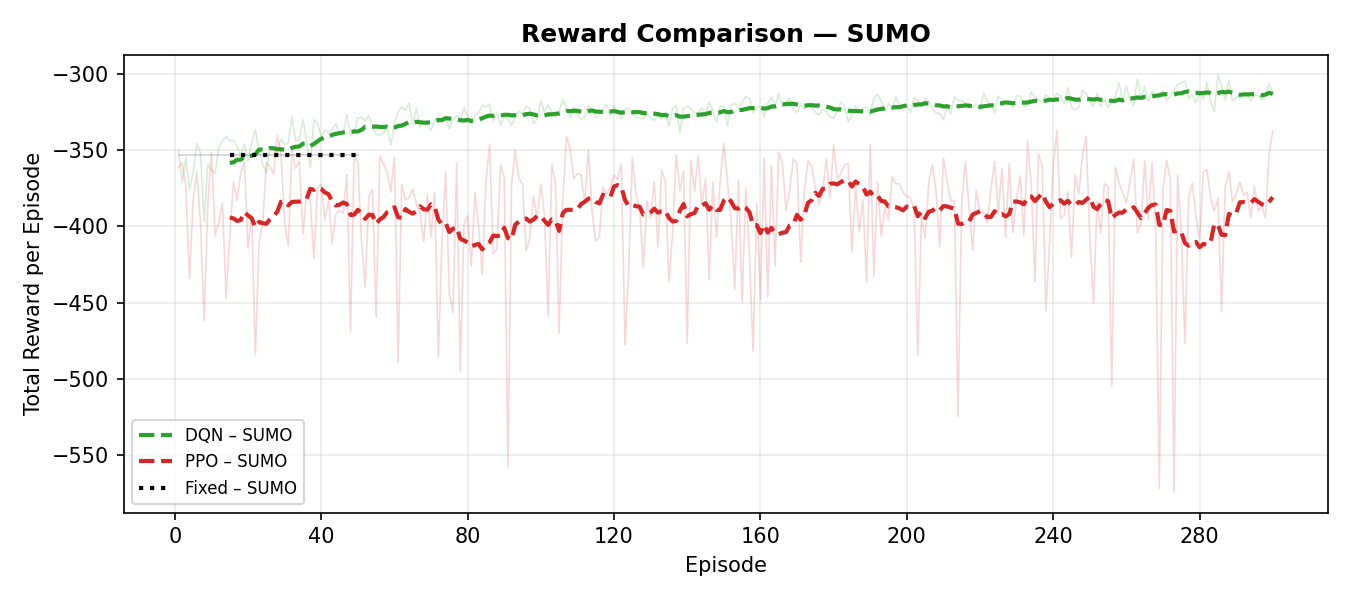
\includegraphics[width=\textwidth]{results/comparison_sumo.png}
    \caption{SUMO training curves. DQN converges above fixed-time; PPO degrades.}
    \label{fig:train_sumo}
  \end{minipage}
  \hfill
  \begin{minipage}[b]{0.48\textwidth}
    \centering
    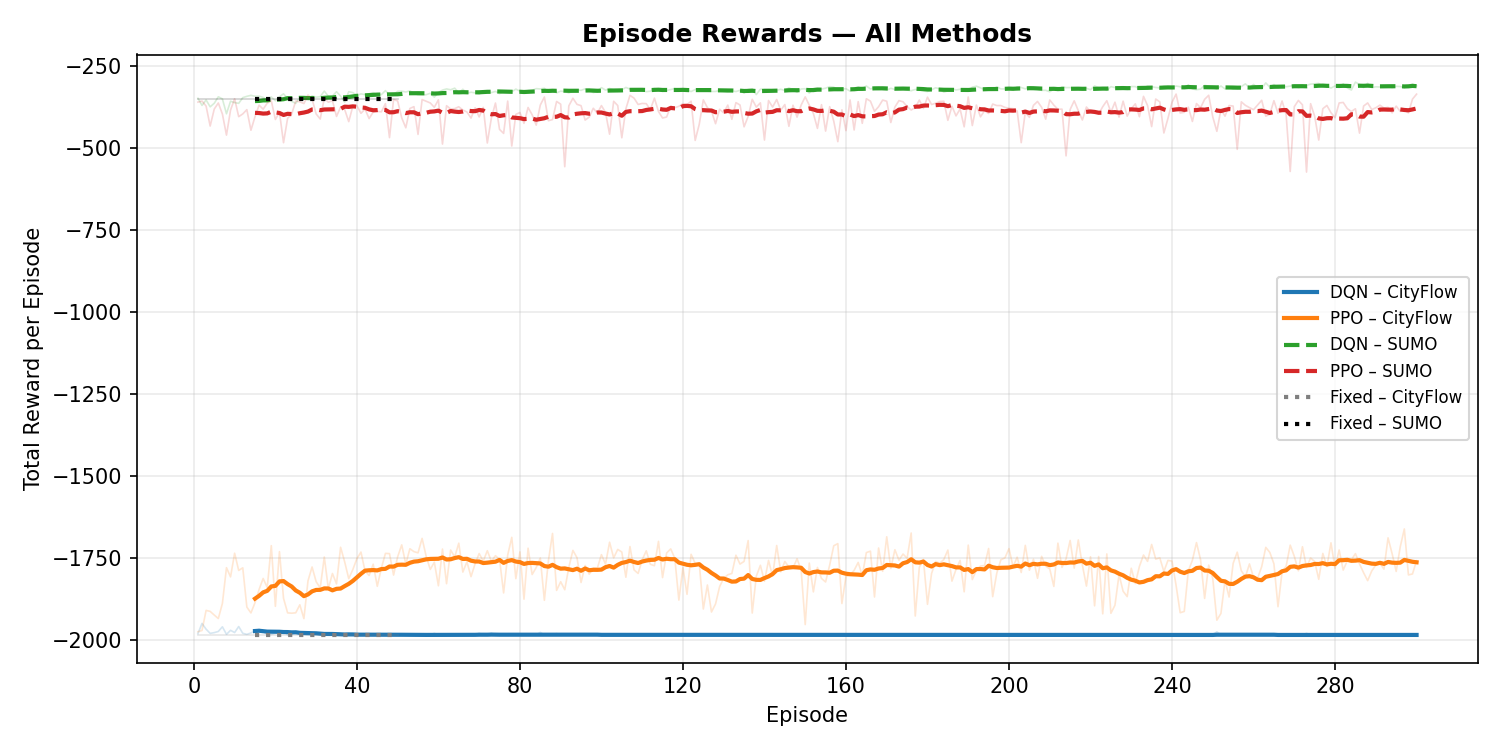
\includegraphics[width=\textwidth]{results/comparison_rewards.png}
    \caption{CityFlow training curves. PPO improves gradually; DQN is flat.}
    \label{fig:train_cityflow}
  \end{minipage}
\end{figure}

\subsection{Final Performance}

Table~\ref{tab:eval} and Figures~\ref{fig:eval_sumo}--\ref{fig:eval_cityflow}
report evaluation metrics over 10 held-out episodes using the best saved
checkpoint ($\varepsilon{=}0$ for DQN).

\begin{table}[H]
\centering
\caption{Evaluation results (10 episodes, best checkpoint).
Queue: mean waiting vehicles per step.
Throughput: vehicles completing route per episode (SUMO only).}
\label{tab:eval}
\begin{tabular}{lrrrrr}
\toprule
 & \multicolumn{3}{c}{\textbf{SUMO (moderate load)}} &
   \multicolumn{2}{c}{\textbf{CityFlow (near-saturation)}} \\
\cmidrule(lr){2-4}\cmidrule(lr){5-6}
\textbf{Method} & Reward & Queue & Throughput & Reward & Queue \\
\midrule
Fixed-time & $-352.9$ & $6.03$ & $1{,}018$ & $-1982.4$ & $449.6$ \\
DQN  & $\mathbf{-312.5}$ & $\mathbf{3.24}$ & $\mathbf{1{,}134}$ & $-1983.6$ & $446.6$ \\
PPO  & $-374.2$ & $7.60$ & $1{,}112$ & $\mathbf{-1791.9}$ & $469.6$ \\
\bottomrule
\end{tabular}
\end{table}

\begin{figure}[H]
  \centering
  \begin{minipage}[b]{0.48\textwidth}
    \centering
    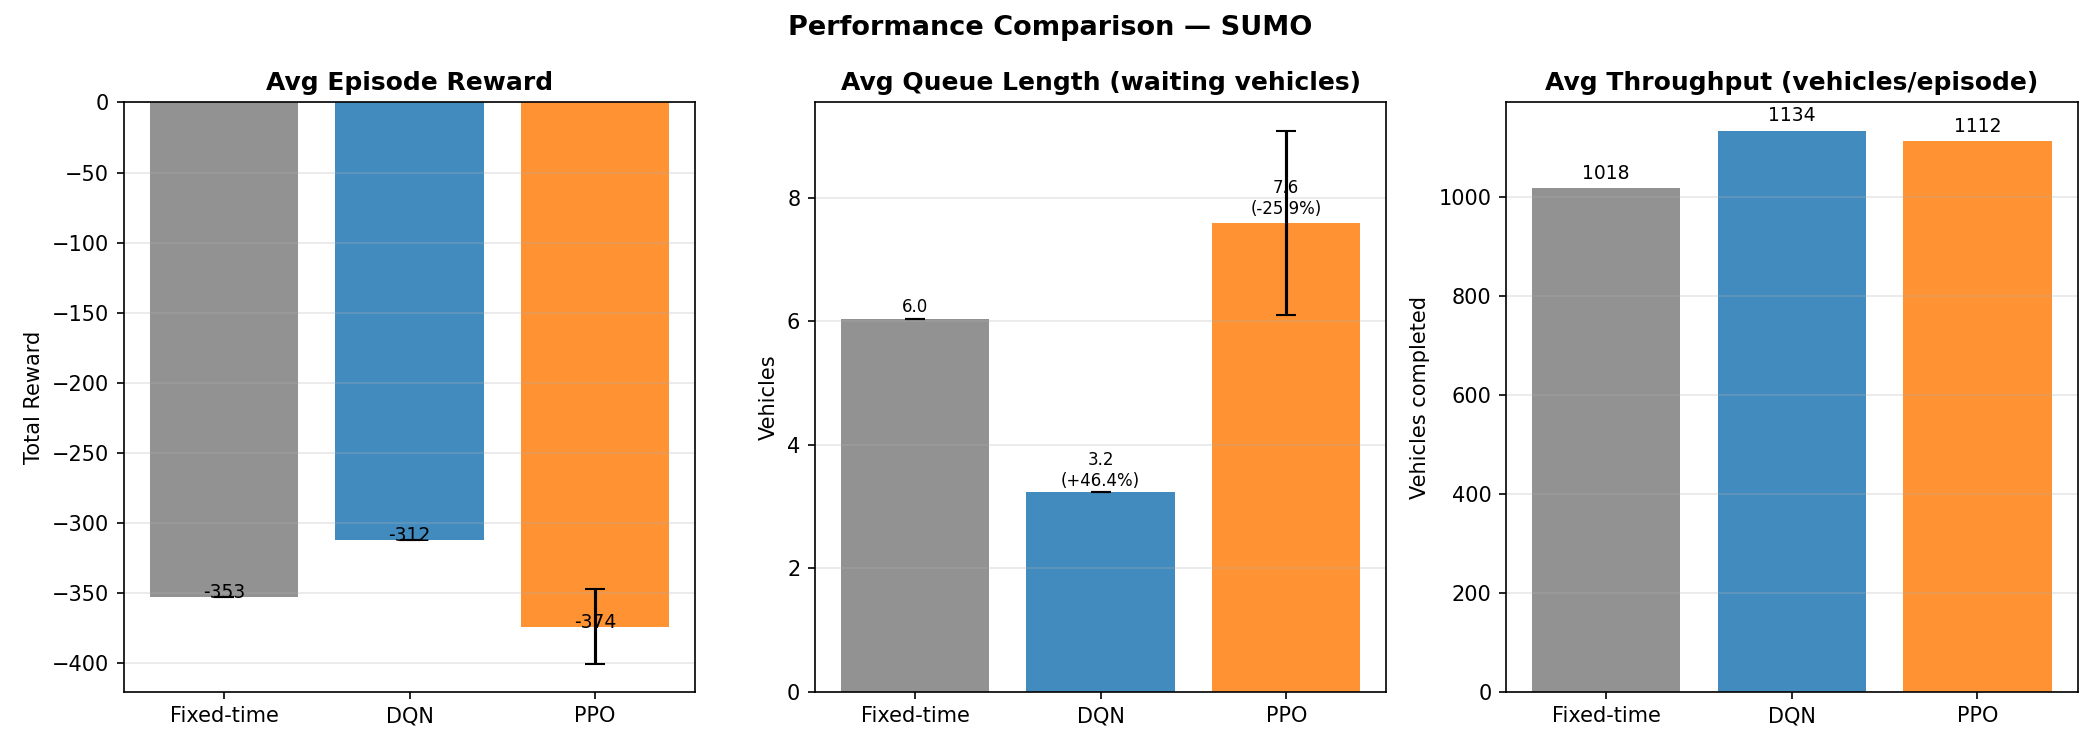
\includegraphics[width=\textwidth]{results/evaluation_sumo.png}
    \caption{SUMO evaluation. DQN leads on all three metrics.}
    \label{fig:eval_sumo}
  \end{minipage}
  \hfill
  \begin{minipage}[b]{0.48\textwidth}
    \centering
    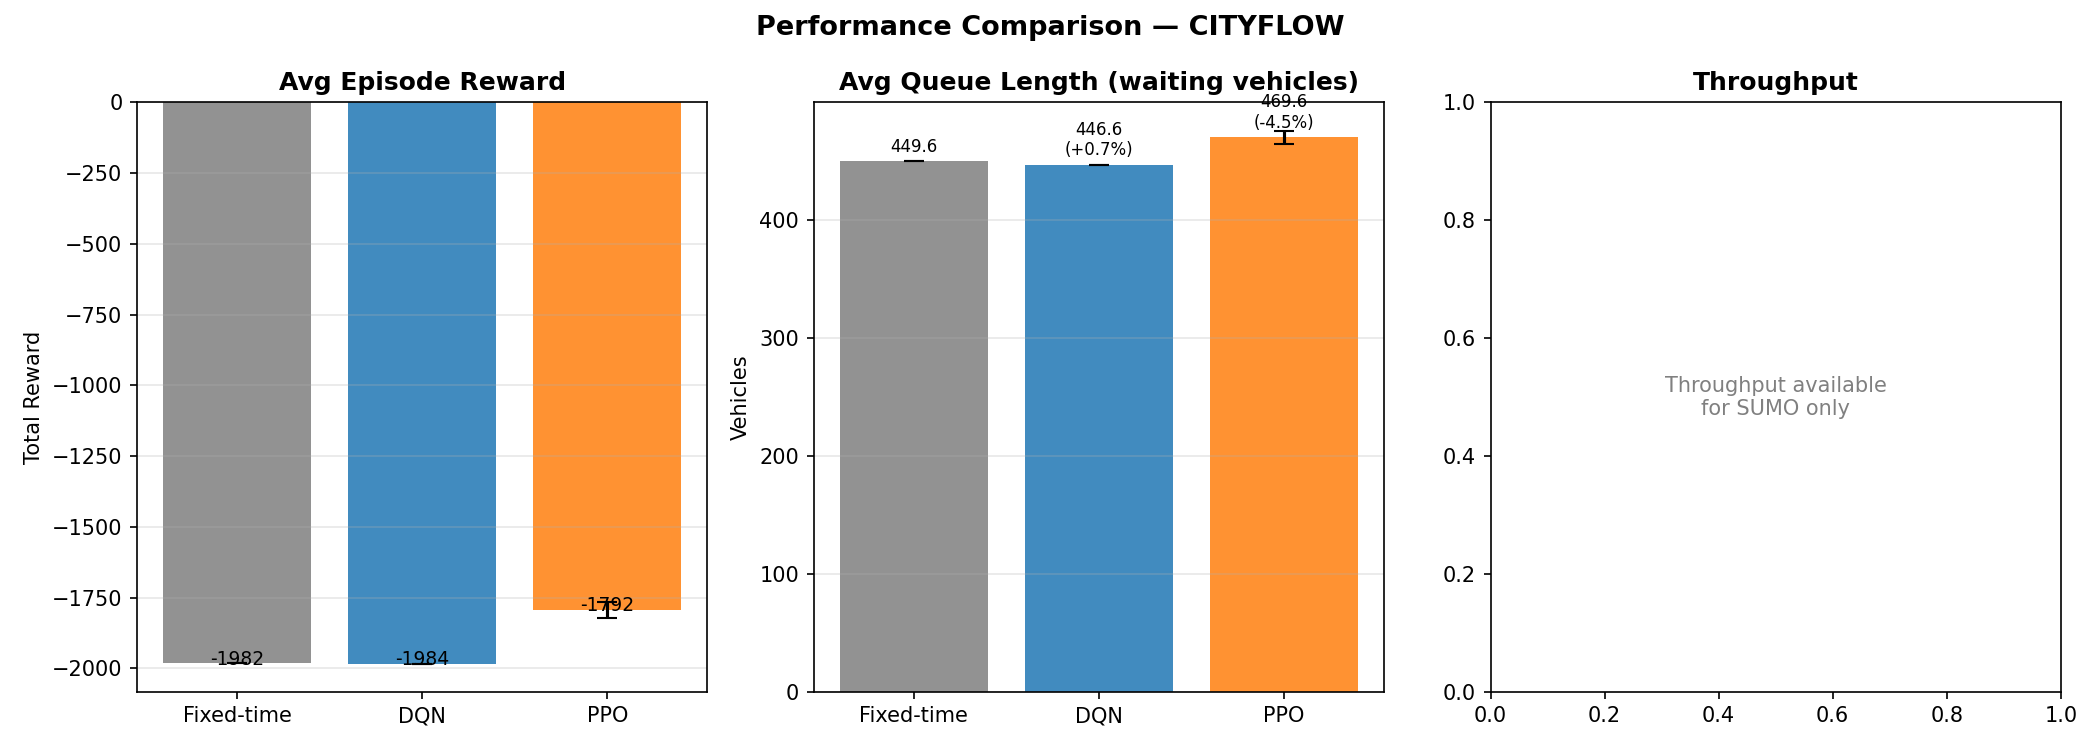
\includegraphics[width=\textwidth]{results/evaluation_cityflow.png}
    \caption{CityFlow evaluation. PPO achieves best reward; DQN matches fixed.}
    \label{fig:eval_cityflow}
  \end{minipage}
\end{figure}

\paragraph{SUMO (moderate load).}
DQN achieves a \textbf{11.4\%} reward improvement ($-312.5$ vs.\ $-352.9$),
a \textbf{46.3\%} reduction in queue length ($3.24$ vs.\ $6.03$ waiting
vehicles), and an \textbf{11.4\%} throughput increase ($1{,}134$ vs.\
$1{,}018$ vehicles/episode).  The off-policy replay buffer is the deciding
factor: by recycling thousands of past transitions, DQN learns that holding the
heavier-queue direction for longer — rather than alternating mechanically —
substantially reduces total waiting.

PPO on SUMO ends \emph{below} the fixed baseline ($-374$ vs.\ $-352$).
Without a replay buffer, on-policy gradient updates struggle with the delayed,
low-variance reward structure; the agent never stabilises a consistent policy.

\paragraph{CityFlow (near-saturation).}
When both approaches are perpetually congested, the advantage of adaptive
switching shrinks: there is no clearly dominant direction, so the fixed plan
performs nearly as well as any binary policy can.  DQN's Q-values converge
to nearly identical estimates for both actions, effectively degenerating to
a fixed policy.  PPO's advantage estimates, being relative rather than
absolute, retain a weak but exploitable signal, yielding a \textbf{9.6\%}
reward gain ($-1791$ vs.\ $-1982$) with high variance across episodes.

\subsection{Signal Phase Analysis}

Figure~\ref{fig:phases} shows phase decisions over 200 steps on SUMO.  The
fixed controller alternates every 30 steps without exception.  DQN holds
phases adaptively: when one direction builds a queue, it extends the green
until the backlog clears, then switches promptly — qualitatively matching
the max-pressure policy of \citet{wei2019presslight}.  PPO switches far more
frequently, often within a single 10-step action period; the resulting
yellow-transition overhead consumes effective green time and degrades performance.

\begin{figure}[H]
  \centering
  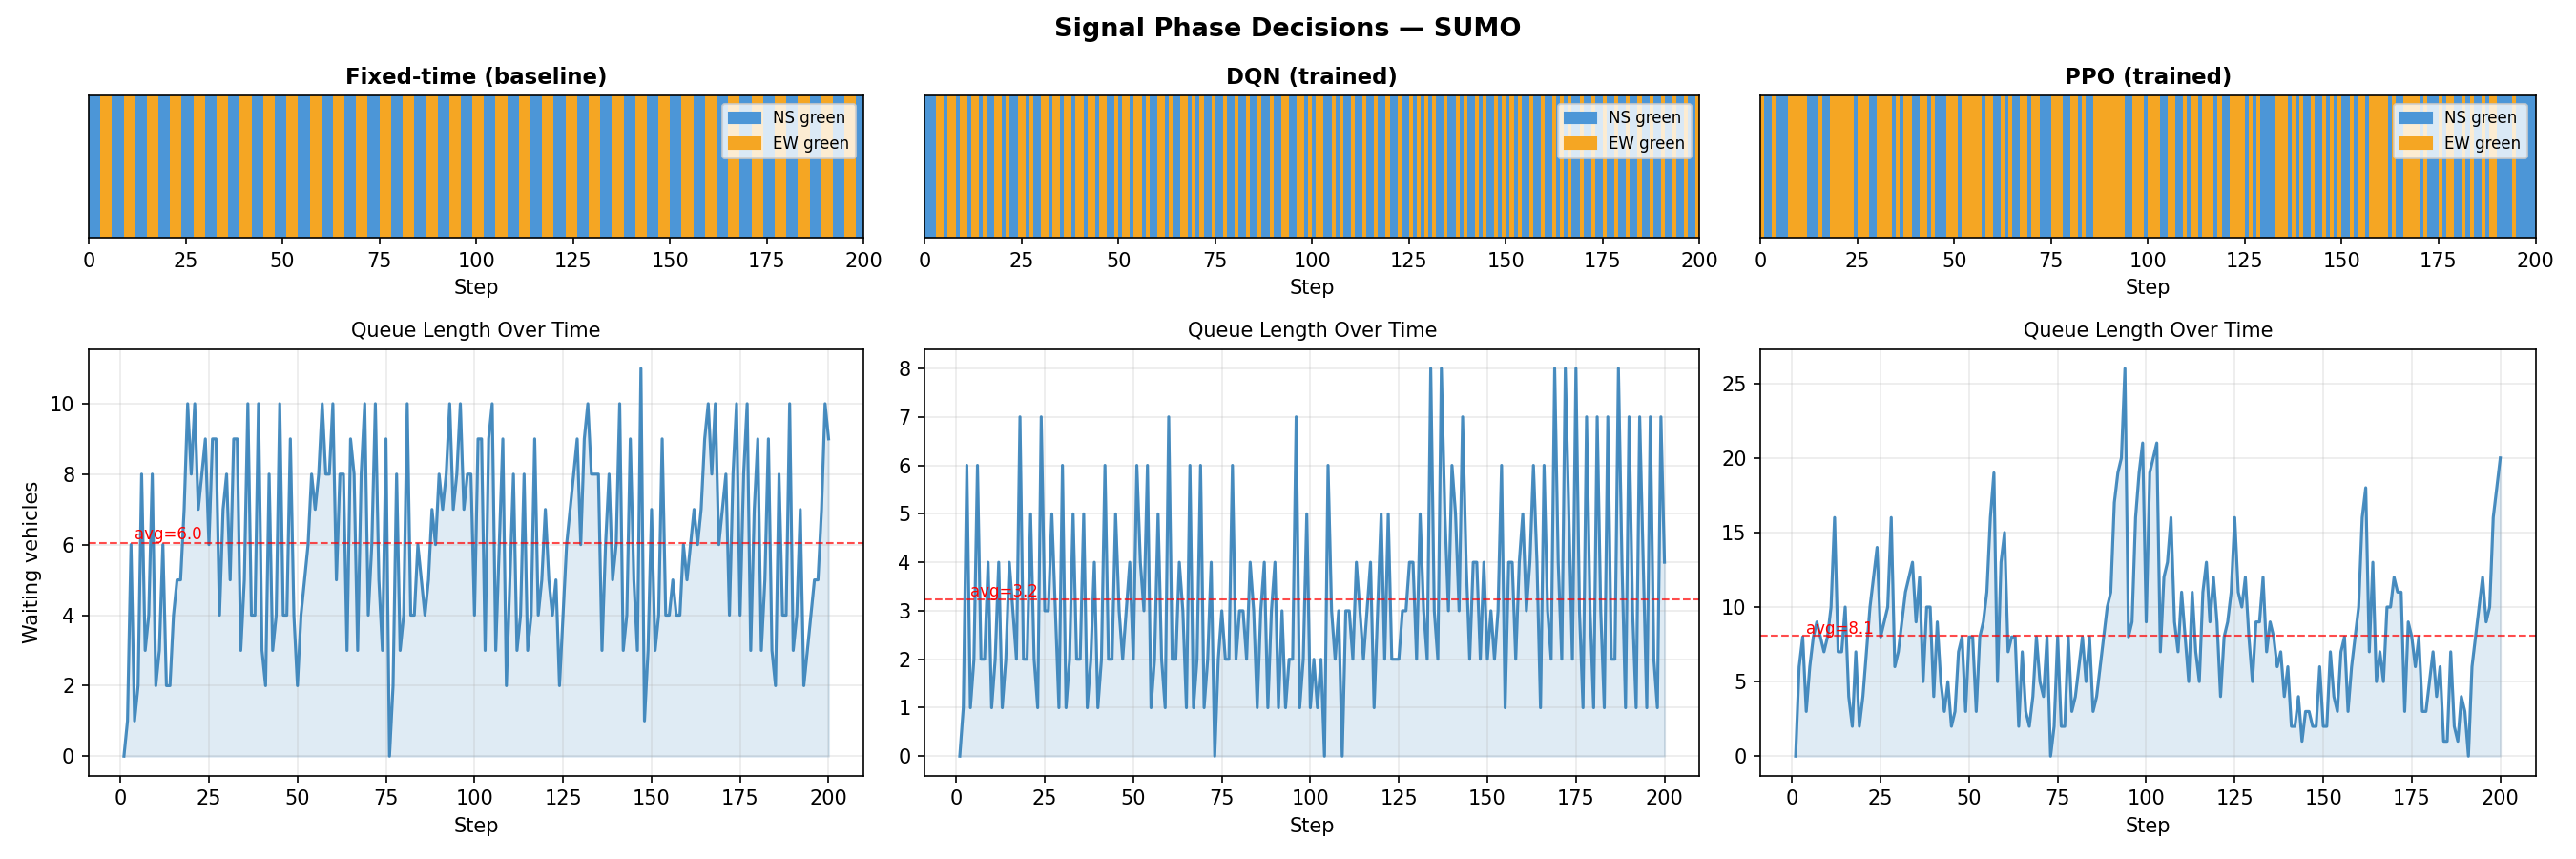
\includegraphics[width=0.72\textwidth]{results/phase_timeline_sumo.png}
  \caption{Phase decisions and queue traces over 200 steps (SUMO).
  \textbf{Top}: fixed-time (rigid 30-step alternation).
  \textbf{Middle}: DQN (adaptive — holds dominant phase until queue clears).
  \textbf{Bottom}: PPO (excessive switching, high yellow-transition overhead).}
  \label{fig:phases}
\end{figure}

% ── 5. Conclusion ─────────────────────────────────────────────────────────────
\section{Conclusion}

\paragraph{Can RL effectively tackle adaptive signal control?}
The answer is \emph{yes, under moderate load}: DQN reduces queue length by
46\% and increases throughput by 11\% on SUMO, demonstrating that a small
neural network can learn the core insight — serve the heavier queue — directly
from experience.  Under near-saturation (CityFlow), the benefit shrinks because
both phases are perpetually congested; here PPO ekes out a 9.6\% reward gain
while DQN degenerates.  The practical takeaway is that adaptive RL control
delivers the most value precisely in the regimes where fixed plans are most
obviously broken: moderate and highly variable load.

\paragraph{Limitations.}
Both agents operate on a single isolated intersection with symmetric, stationary
demand and a binary action space.  The binary space cannot express fractional
green splits or more than two phases, and neither agent was evaluated under
dynamic conditions such as incidents or time-varying demand.

\paragraph{Future work.}
\begin{itemize}
  \item \textbf{Multi-intersection MARL}: extend to a grid with graph
        attention coordination~\citep{wei2019colight}, where the single-intersection
        policy serves as the per-node base agent.
  \item \textbf{Variable phase durations}: augment the action space to include
        the green duration, not just which phase to serve.
  \item \textbf{Pressure-based reward}: replace Equation~\ref{eq:reward} with
        a pressure signal~\citep{wei2019presslight} to improve convergence under
        saturation.
  \item \textbf{Real-world validation}: calibrate SUMO demand from loop-detector
        logs to test generalization beyond synthetic scenarios.
\end{itemize}

\acks{Code and trained models:
\url{https://github.com/ashzyc/CS9170-RL-Traffic-Efficiency}.
All experiments ran on a standard laptop CPU; no external funding was received.}

\bibliography{references}

\end{document}
